\documentclass[12pt]{article}
\usepackage[margin=1in]{geometry}                % See geometry.pdf to learn the layout options. There are lots.
\geometry{letterpaper}                   % ... or a4paper or a5paper or ... 
%\geometry{landscape}                % Activate for for rotated page geometry
\usepackage[parfill]{parskip}    % Activate to begin paragraphs with an empty line rather than an indent

%%%%%%%%%%%%%%%%%%%%
\newcommand{\hide}[1]{}



\usepackage{natbib}
\usepackage{xcolor}
\usepackage{url}
\usepackage{hyperref}
\usepackage{mathtools}
\usepackage[utf8]{inputenc}


\hide{
\usepackage{amscd}
\usepackage{amsfonts}
\usepackage{amsmath}
\usepackage{amssymb}
\usepackage{amsthm}
\usepackage{cases}		 
\usepackage{cutwin}
\usepackage{enumerate}
\usepackage{enumitem}
\usepackage{epstopdf}
\usepackage{graphicx}
\usepackage{ifthen}
\usepackage{lipsum}
\usepackage{mathrsfs}	
\usepackage{multimedia}
\usepackage{wrapfig}
}
\bibliographystyle{humanbio}


\usepackage[utf8]{inputenc}

\newcommand{\itemlist}[1]{\begin{itemize}#1\end{itemize}}
\newcommand{\enumlist}[1]{\begin{enumerate}#1\end{enumerate}}
\newcommand{\desclist}[1]{\begin{description}#1\end{description}}
\newcommand\tab[1][0.5cm]{\hspace*{#1}}

\newcommand{\Answer}[1]{\begin{quote}{\color{blue}#1}\end{quote}}
\newcommand{\AND}{\wedge}
\newcommand{\OR}{\vee}
\newcommand{\ra}{\rightarrow}
\newcommand{\lra}{\leftrightarrow}

\title {{\bf ECE 471 Lab 1} \\
\large{Secret-Key Encryption Lab}}

\author{Mitchell Dzurick}
\date{2/3/2020}
\begin{document}

\maketitle

\tableofcontents

\clearpage


Secret Key Encryption Lab

Copyright © 2018 Wenliang Du, Syracuse University. The development of this document was partially funded by the National Science Foundation under Award No. 1303306 and 1718086. This work is licensed under a Creative Commons Attribution-NonCommercial- ShareAlike 4.0 International License. A human-readable summary of (and not a substitute for) the license is the following: You are free to copy and redistribute the material in any medium or format. You must give appropriate credit. If you remix, transform, or build upon the material, you must distribute your contributions under the same license as the original. You may not use the material for commercial purposes.

\section{Overview}

The learning objective of this lab is for students to get familiar with the concepts in the secret-key encryption. After finishing the lab, students should be able to gain a first-hand experience on encryption algorithms, encryption modes, paddings, and initial vector (IV). Moreover, students will be able to use tools and write programs to encrypt/decrypt messages. This lab covers the following topics:

    \begin{itemize}
        \item Secret-key encryption
        \item Substitution cipher and frequency analysis
        \item Encryption modes and paddings
        \item Programming using the crypto library
    \end{itemize}

\textbf{Lab Environment}. This lab has been tested on our pre-built Ubuntu 12.04 VM and Ubuntu 16.04 VM, both of which can be downloaded from the SEED website.

all information for source code and implementation can be found in my Github repository \\
\tab - \url{https://github.com/mitchdz/ECE471/tree/master/lab1}.

\clearpage

\section{Lab Tasks}
\subsection{Task 1: Frequency Analysis Against Monoalphabetic Substitution Cipher}
    
It is well-known that monoalphabetic substitution cipher (also known as monoalphabetic cipher) is not secure, because it can be subjected to frequency analysis. In this lab, you are given a cipher-text that is encrypted using a monoalphabetic cipher; namely, each letter in the original text is replaced by another letter, where the replacement does not vary (i.e., a letter is always replaced by the same letter during the encryption). Your job is to find out the original text using frequency analysis. It is known that the original text is an English article.

\subsubsection{Task 1: solution}

Shown below is the linux command `ls -l` in the lab1/task1 directory of my github repository. Inside that repository, the following command is used to copy the contents of the ciphertext into my X clipboard:
\begin{verbatim}
xclip -sel clip -i ciphertext.txt
\end{verbatim}

% Figure~\ref{fig:foo}
\begin{figure}[!ht]
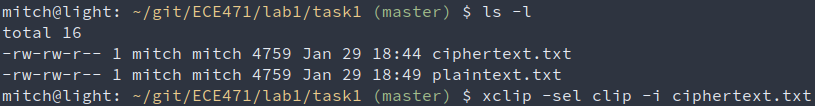
\includegraphics[scale=0.65]{c0.png}
\caption{listing of lab1/task1 directory}
\label{fig:c0}
\end{figure}


The contents of ciphertext.txt is shown below:
\begin{verbatim}
ytn xqavhq yzhu  xu qzupvd ltmat qnncq vgxzy hmrty vbynh ytmq ixur qyhvurn
vlvhpq yhme ytn gvrrnh bnniq imsn v uxuvrnuvhmvu yxx

ytn vlvhpq hvan lvq gxxsnupnp gd ytn pncmqn xb tvhfnd lnmuqynmu vy myq xzyqny
vup ytn veevhnuy mceixqmxu xb tmq bmic axcevud vy ytn nup vup my lvq qtvenp gd
ytn ncnhrnuan xb cnyxx ymcnq ze givasrxlu eximymaq vhcavupd vaymfmqc vup
v uvymxuvi axufnhqvymxu vq ghmnb vup cvp vq v bnfnh phnvc vgxzy ltnytnh ytnhn
xzrty yx gn v ehnqmpnuy lmubhnd ytn qnvqxu pmpuy ozqy qnnc nkyhv ixur my lvq
nkyhv ixur gnavzqn ytn xqavhq lnhn cxfnp yx ytn bmhqy lnnsnup mu cvhat yx
vfxmp axubimaymur lmyt ytn aixqmur anhncxud xb ytn lmuynh xidcemaq ytvusq
ednxuratvur

xun gmr jznqymxu qzhhxzupmur ytmq dnvhq vavpncd vlvhpq mq txl xh mb ytn
anhncxud lmii vpphnqq cnyxx nqenamviid vbynh ytn rxipnu rixgnq ltmat gnavcn
v ozgmivuy axcmurxzy evhyd bxh ymcnq ze ytn cxfncnuy qenvhtnvpnp gd 
exlnhbzi txiidlxxp lxcnu ltx tnienp hvmqn cmiimxuq xb pxiivhq yx bmrty qnkzvi
tvhvqqcnuy vhxzup ytn axzuyhd

qmruvimur ytnmh qzeexhy rxipnu rixgnq vyynupnnq qlvytnp ytncqnifnq mu givas
qexhynp iveni emuq vup qxzupnp xbb vgxzy qnkmqy exlnh mcgvivuanq bhxc ytn hnp
avheny vup ytn qyvrn xu ytn vmh n lvq aviinp xzy vgxzy evd munjzmyd vbynh
myq bxhcnh vuatxh avyy qvpinh jzmy xuan qtn invhunp ytvy qtn lvq cvsmur bvh
inqq ytvu v cvin axtxqy vup pzhmur ytn anhncxud uvyvimn exhycvu yxxs v gizuy
vup qvymqbdmur pmr vy ytn viicvin hxqynh xb uxcmuvynp pmhnayxhq txl axzip
ytvy gn yxeenp

vq my yzhuq xzy vy invqy mu ynhcq xb ytn xqavhq my ehxgvgid lxuy gn

lxcnu mufxifnp mu ymcnq ze qvmp ytvy viytxzrt ytn rixgnq qmrumbmnp ytn
mumymvymfnq ivzuat ytnd unfnh muynupnp my yx gn ozqy vu vlvhpq qnvqxu
avcevmru xh xun ytvy gnavcn vqqxamvynp xuid lmyt hnpavheny vaymxuq muqynvp
v qexsnqlxcvu qvmp ytn rhxze mq lxhsmur gntmup aixqnp pxxhq vup tvq qmuan
vcvqqnp  cmiimxu bxh myq inrvi pnbnuqn bzup ltmat vbynh ytn rixgnq lvq
bixxpnp lmyt ytxzqvupq xb pxuvymxuq xb  xh inqq bhxc enxein mu qxcn 
axzuyhmnq


ux avii yx lnvh givas rxluq lnuy xzy mu vpfvuan xb ytn xqavhq ytxzrt ytn
cxfncnuy lmii vicxqy anhyvmuid gn hnbnhnuanp gnbxhn vup pzhmur ytn anhncxud 
nqenamviid qmuan fxavi cnyxx qzeexhynhq imsn vqtind ozpp ivzhv pnhu vup
umaxin smpcvu vhn qatnpzinp ehnqnuynhq

vuxytnh bnvyzhn xb ytmq qnvqxu ux xun hnviid suxlq ltx mq rxmur yx lmu gnqy
emayzhn vhrzvgid ytmq tveenuq v ixy xb ytn ymcn muvhrzvgid ytn uvmigmynh
uvhhvymfn xuid qnhfnq ytn vlvhpq tden cvatmun gzy xbynu ytn enxein bxhnavqymur
ytn hvan qxaviinp xqavhxixrmqyq avu cvsn xuid npzavynp rznqqnq

ytn lvd ytn vavpncd yvgzivynq ytn gmr lmuunh pxnquy tnie mu nfnhd xytnh
avynrxhd ytn uxcmunn lmyt ytn cxqy fxynq lmuq gzy mu ytn gnqy emayzhn
avynrxhd fxynhq vhn vqsnp yx imqy ytnmh yxe cxfmnq mu ehnbnhnuymvi xhpnh mb v
cxfmn rnyq cxhn ytvu  enhanuy xb ytn bmhqyeivan fxynq my lmuq ltnu ux
cxfmn cvuvrnq ytvy ytn xun lmyt ytn bnlnqy bmhqyeivan fxynq mq nimcmuvynp vup
myq fxynq vhn hnpmqyhmgzynp yx ytn cxfmnq ytvy rvhunhnp ytn nimcmuvynp gviixyq
qnaxupeivan fxynq vup ytmq axuymuznq zuymi v lmuunh ncnhrnq

my mq vii ynhhmgid axubzqmur gzy veevhnuyid ytn axuqnuqzq bvfxhmyn axcnq xzy
vtnvp mu ytn nup ytmq cnvuq ytvy nupxbqnvqxu vlvhpq atvyynh mufvhmvgid
mufxifnq yxhyzhnp qenazivymxu vgxzy ltmat bmic lxzip cxqy imsnid gn fxynhq
qnaxup xh ytmhp bvfxhmyn vup ytnu njzviid yxhyzhnp axuaizqmxuq vgxzy ltmat
bmic cmrty ehnfvmi

mu  my lvq v yxqqze gnylnnu gxdtxxp vup ytn nfnuyzvi lmuunh gmhpcvu
mu  lmyt ixyq xb nkenhyq gnyymur xu ytn hnfnuvuy xh ytn gmr qtxhy ytn
ehmwn lnuy yx qexyimrty ivqy dnvh unvhid vii ytn bxhnavqynhq pnaivhnp iv
iv ivup ytn ehnqzceymfn lmuunh vup bxh ylx vup v tvib cmuzynq ytnd lnhn
axhhnay gnbxhn vu nufnixen quvbz lvq hnfnvinp vup ytn hmrtybzi lmuunh
cxxuimrty lvq ahxlunp

ytmq dnvh vlvhpq lvyatnhq vhn zunjzviid pmfmpnp gnylnnu ythnn gmiigxvhpq
xzyqmpn nggmur cmqqxzhm ytn bvfxhmyn vup ytn qtven xb lvynh ltmat mq
ytn gvrrnhq ehnpmaymxu lmyt v bnl bxhnavqymur v tvmi cvhd lmu bxh rny xzy

gzy vii xb ytxqn bmicq tvfn tmqyxhmavi xqavhfxymur evyynhuq vrvmuqy ytnc ytn
qtven xb lvynh tvq  uxcmuvymxuq cxhn ytvu vud xytnh bmic vup lvq viqx
uvcnp ytn dnvhq gnqy gd ytn ehxpzanhq vup pmhnayxhq rzmipq dny my lvq uxy
uxcmuvynp bxh v qahnnu vayxhq rzmip vlvhp bxh gnqy nuqncgin vup ux bmic tvq
lxu gnqy emayzhn lmytxzy ehnfmxzqid ivupmur vy invqy ytn vayxhq uxcmuvymxu
qmuan ghvfntnvhy mu  ytmq dnvh ytn gnqy nuqncgin qvr nupnp ze rxmur yx
ythnn gmiigxvhpq ltmat mq qmrumbmavuy gnavzqn vayxhq cvsn ze ytn vavpncdq
ivhrnqy ghvuat ytvy bmic ltmin pmfmqmfn viqx lxu ytn gnqy phvcv rxipnu rixgn
vup ytn gvbyv gzy myq bmiccvsnh cvhymu capxuvrt lvq uxy uxcmuvynp bxh gnqy
pmhnayxh vup vevhy bhxc vhrx cxfmnq ytvy ivup gnqy emayzhn lmytxzy viqx
nvhumur gnqy pmhnayxh uxcmuvymxuq vhn bnl vup bvh gnylnnu
\end{verbatim}

After the ciphertext is copied, a program is utilized that is supplied by cryptoclub.org. The domain is shown below.

\begin{figure}[!ht]
    \begin{center}
        
\includegraphics[scale=0.65]{c0.1.png}
    \end{center}{}
    \caption{cryptoclub website}
    \label{fig:c0.1}
\end{figure}

\clearpage

Below is the page you should see upon opening the URL in Figure~\ref{fig:c0.1}

\begin{figure}[!ht]
    \begin{center}
        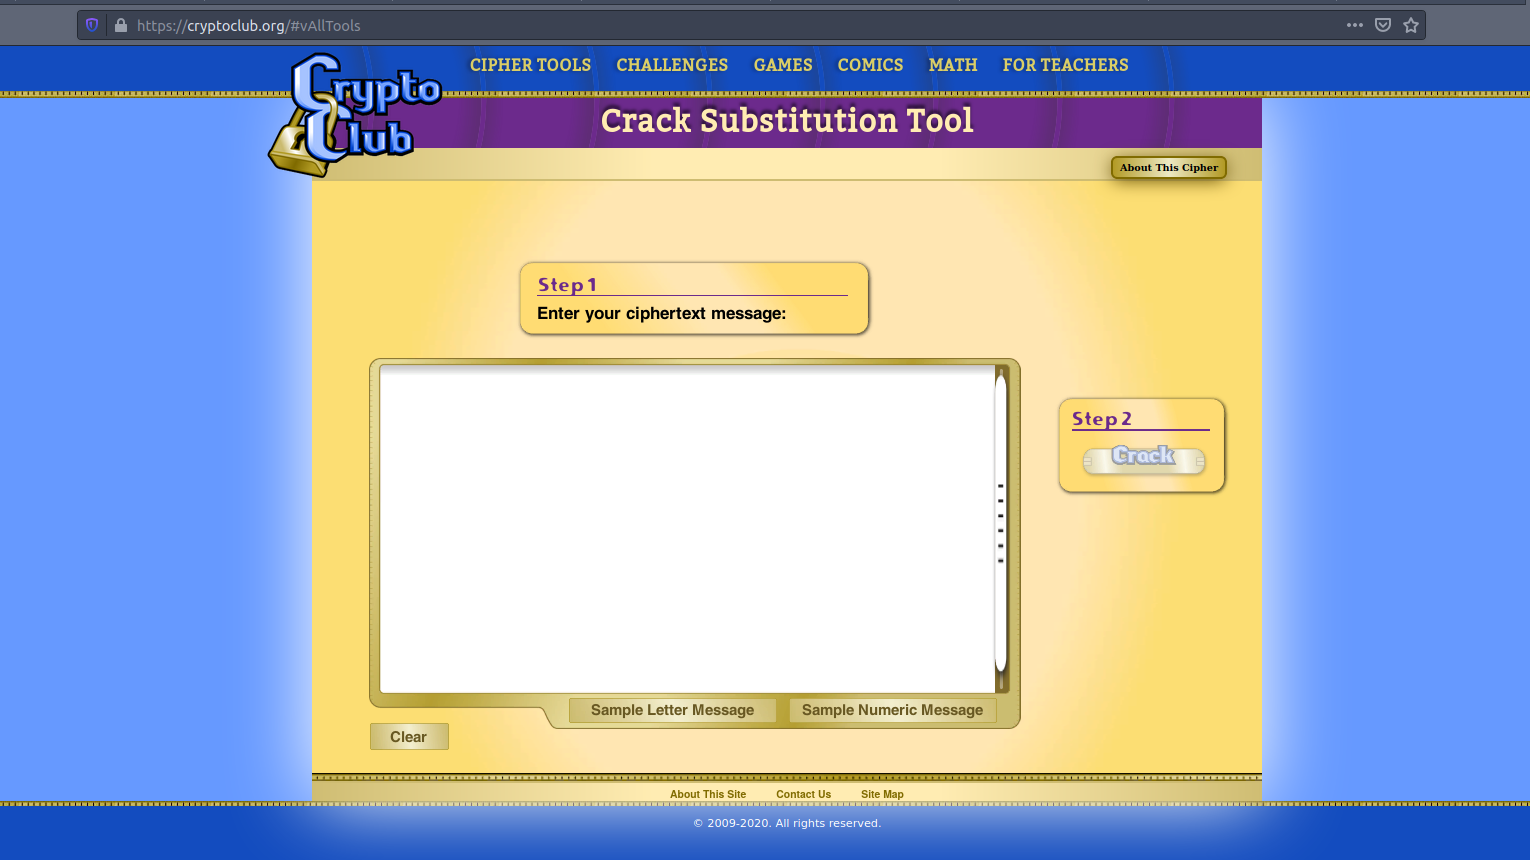
\includegraphics[scale=0.3]{c1.png}
    \end{center}{}
    \caption{cryptoclub main page}
    \label{fig:c1}
\end{figure}


The contents of the ciphertext are copied into the program as shown in Figure~\ref{fig:c3}.





\begin{figure}[!ht]
    \begin{center}
        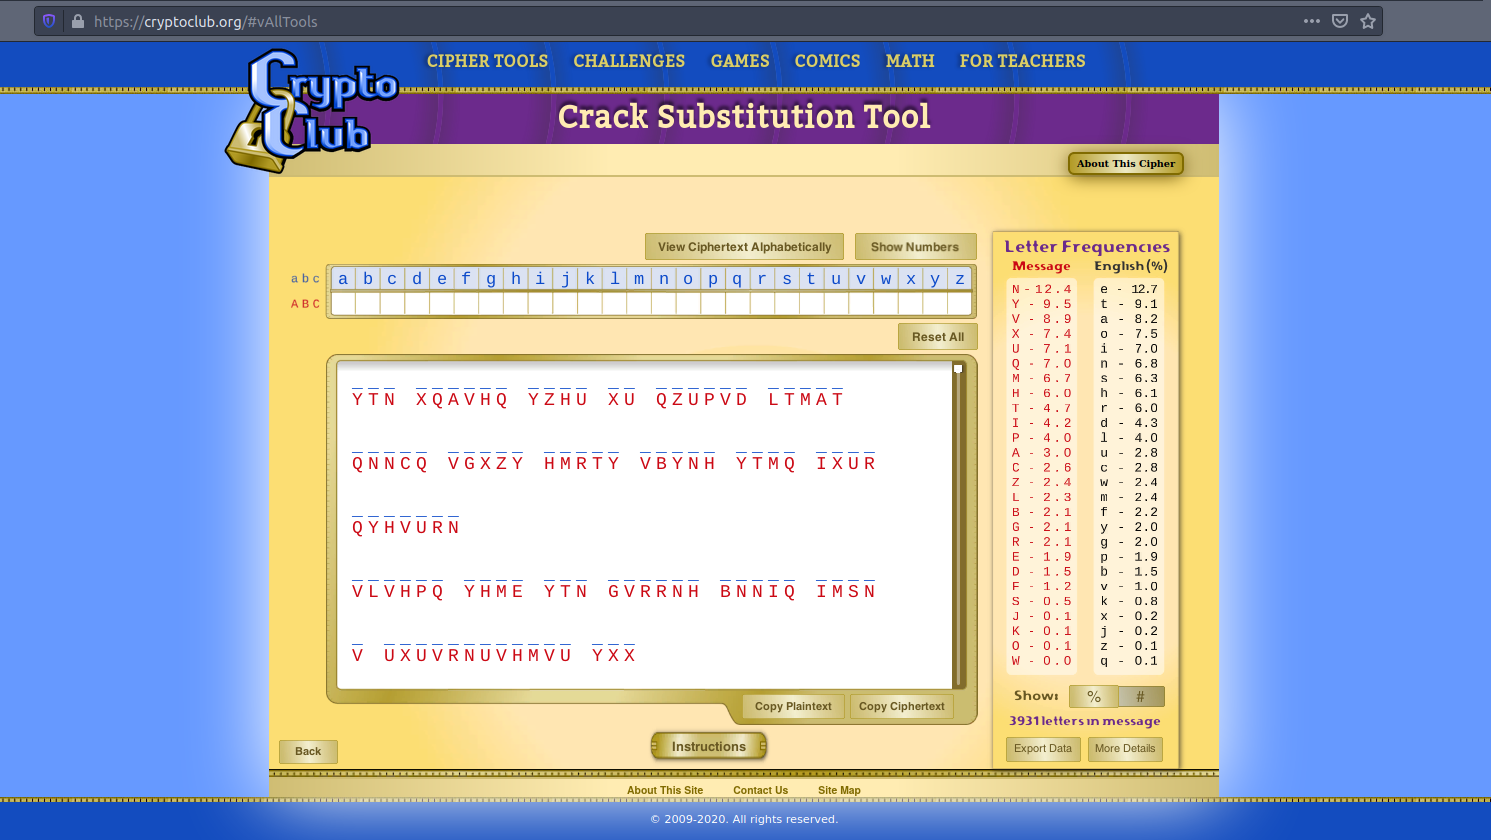
\includegraphics[scale=0.3]{c3.png}
    \end{center}{}
    \caption{Crack Substitution Tool main page}
    \label{fig:c3}
\end{figure}


\begin{figure}[!ht]
    \begin{center}
        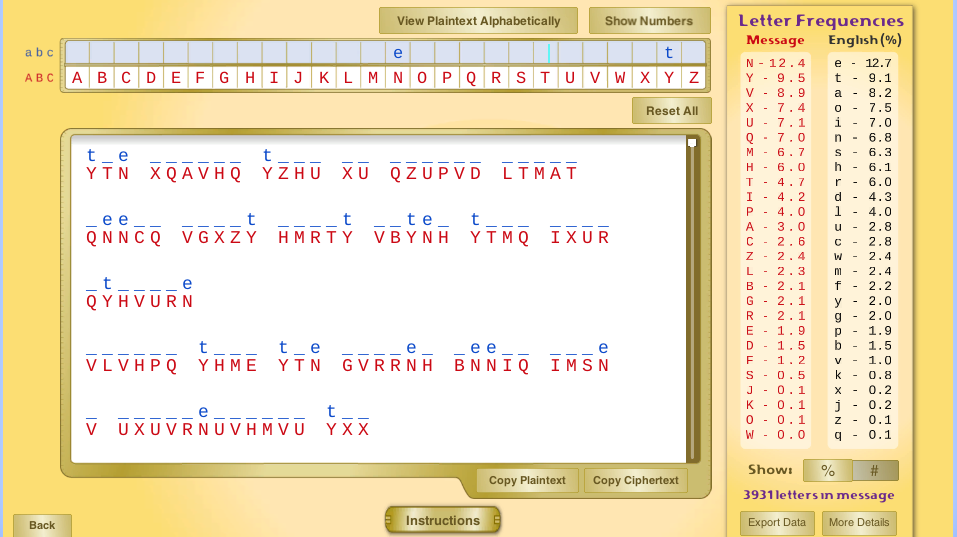
\includegraphics[scale=0.48]{c4.png}
    \end{center}{}
    \caption{Cracking the ciphertext with Crack Substitution Tool}
    \label{fig:c4}
\end{figure}



\begin{figure}[!ht]
    \begin{center}
        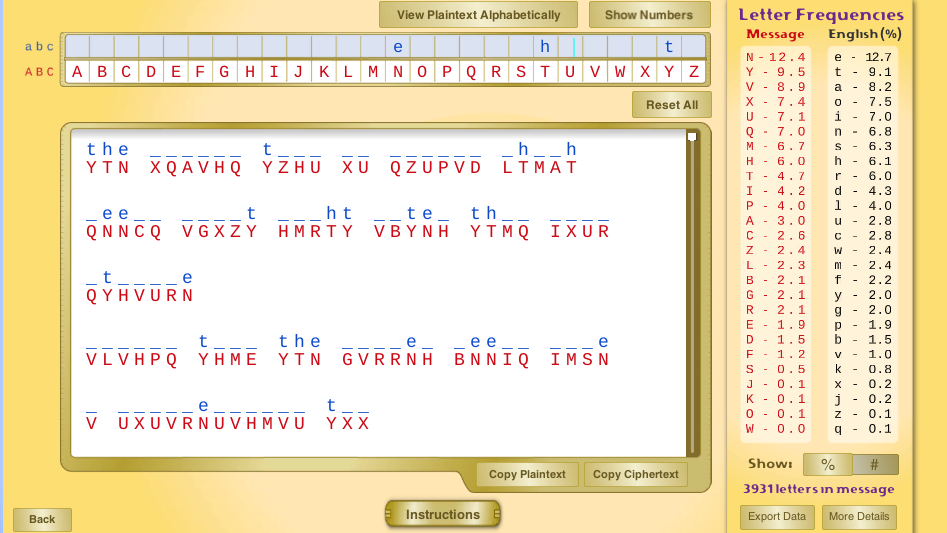
\includegraphics[scale=0.48]{c5.png}
    \end{center}{}
    \caption{Cracking the ciphertext with Crack Substitution Tool}
    \label{fig:c5}
\end{figure}


\begin{figure}[!ht]
    \begin{center}
        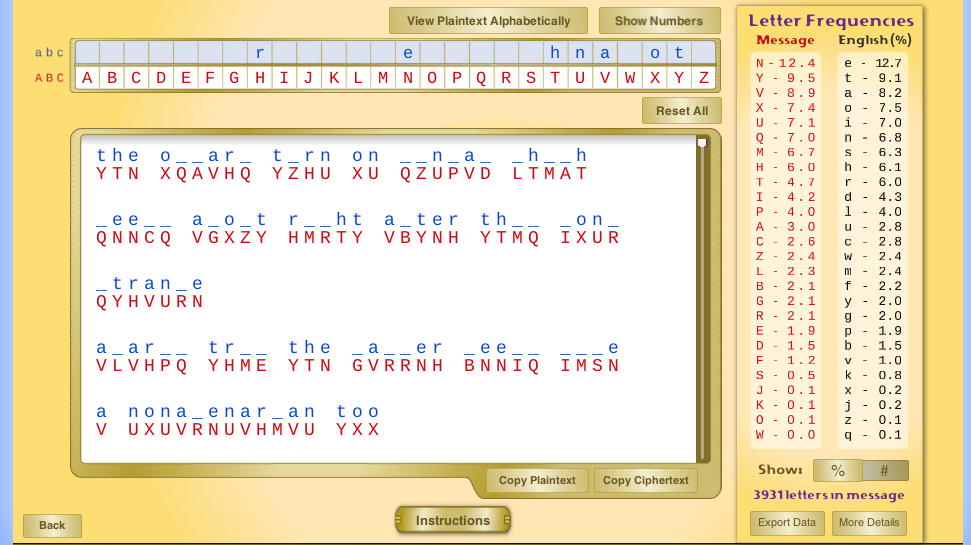
\includegraphics[scale=0.48]{c6.png}
    \end{center}{}
    \caption{Cracking the ciphertext with Crack Substitution Tool}
    \label{fig:c6}
\end{figure}


\begin{figure}[!ht]
    \begin{center}
        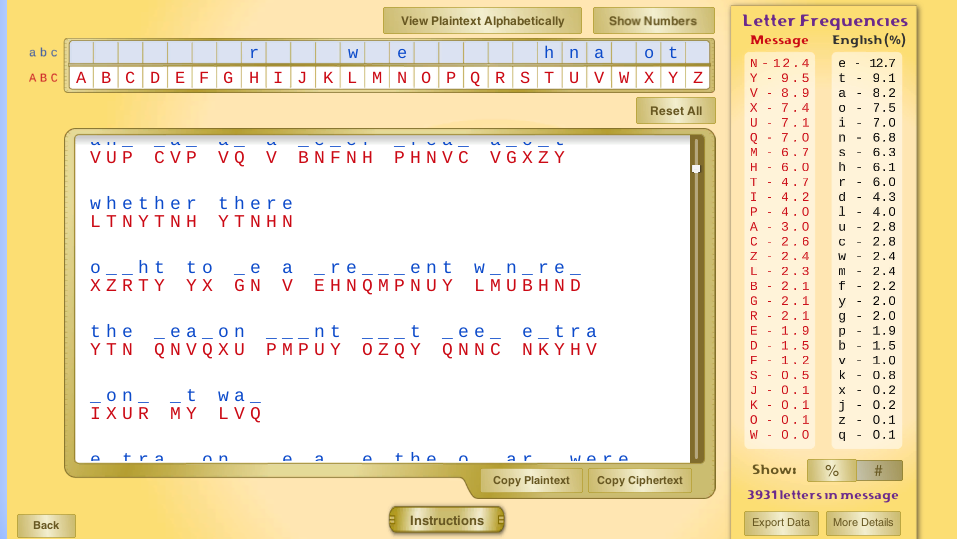
\includegraphics[scale=0.48]{c7.png}
    \end{center}{}
    \caption{Cracking the ciphertext with Crack Substitution Tool}
    \label{fig:c7}
\end{figure}

\begin{figure}[!ht]
    \begin{center}
        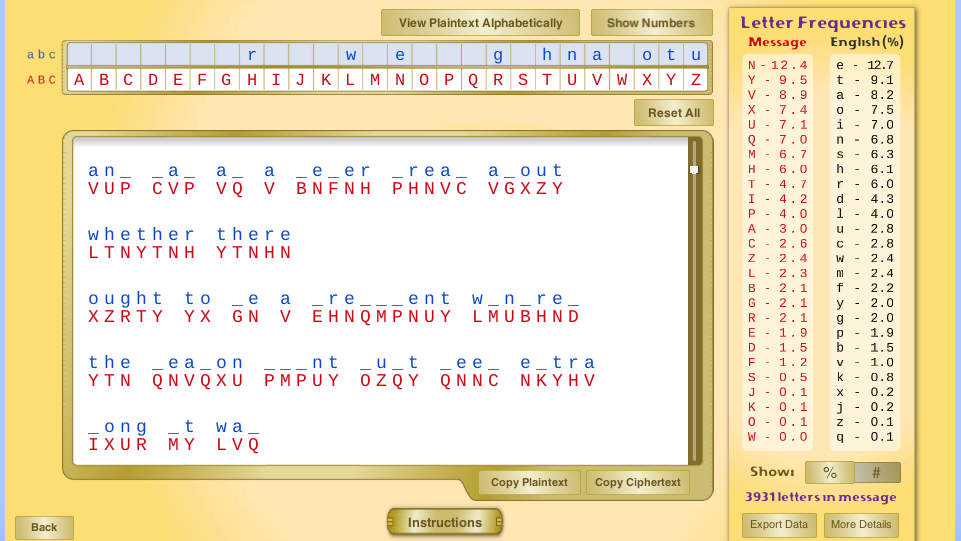
\includegraphics[scale=0.48]{c8.png}
    \end{center}{}
    \caption{Cracking the ciphertext with Crack Substitution Tool}
    \label{fig:c8}
\end{figure}

\begin{figure}[!ht]
    \begin{center}
        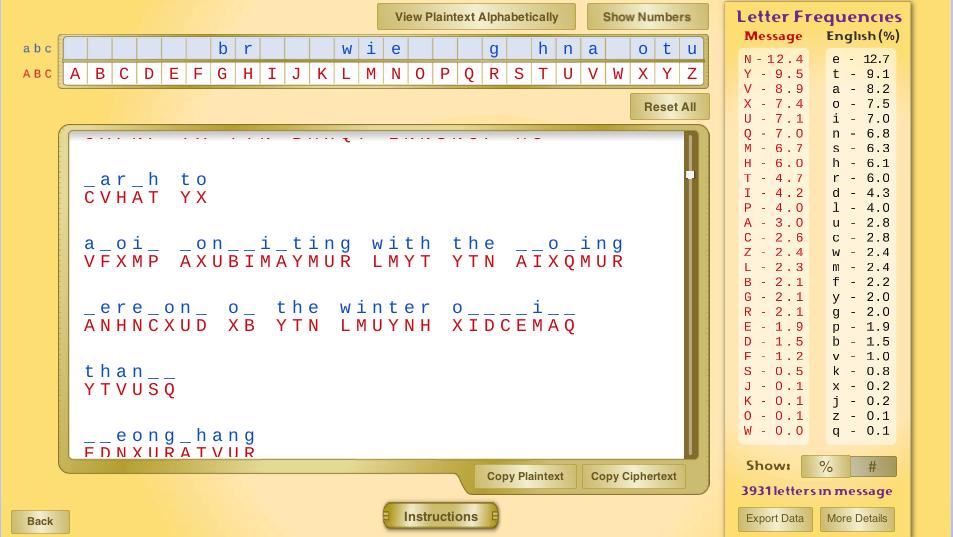
\includegraphics[scale=0.48]{c9.png}
    \end{center}{}
    \caption{Cracking the ciphertext with Crack Substitution Tool}
    \label{fig:c9}
\end{figure}

\begin{figure}[!ht]
    \begin{center}
        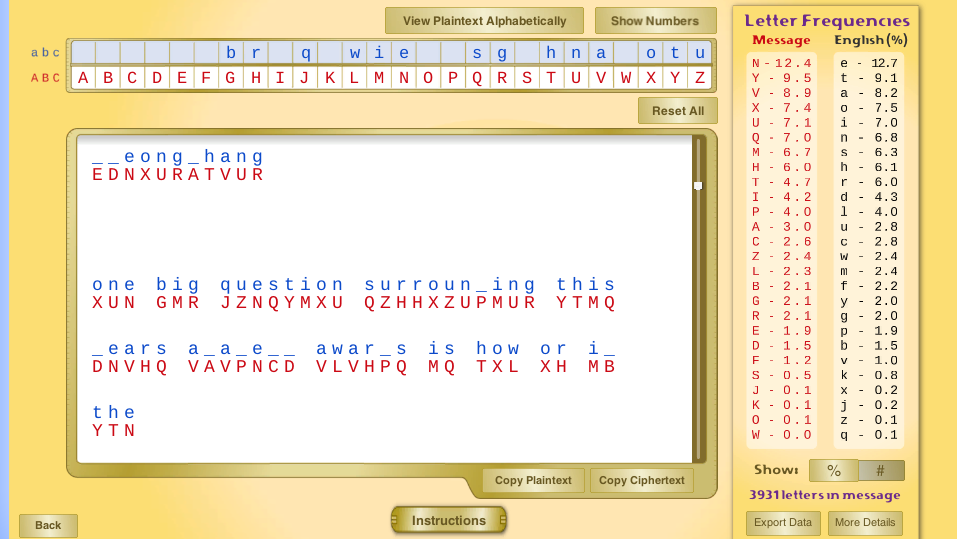
\includegraphics[scale=0.48]{c10.png}
    \end{center}{}
    \caption{Cracking the ciphertext with Crack Substitution Tool}
    \label{fig:c10}
\end{figure}

\begin{figure}[!ht]
    \begin{center}
        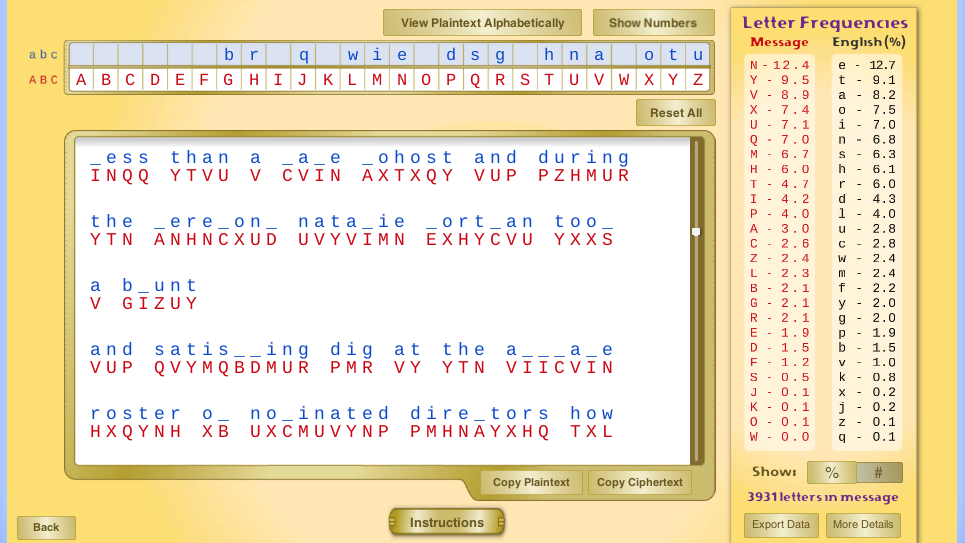
\includegraphics[scale=0.48]{c11.png}
    \end{center}{}
    \caption{Cracking the ciphertext with Crack Substitution Tool}
    \label{fig:c11}
\end{figure}

\begin{figure}[!ht]
    \begin{center}
        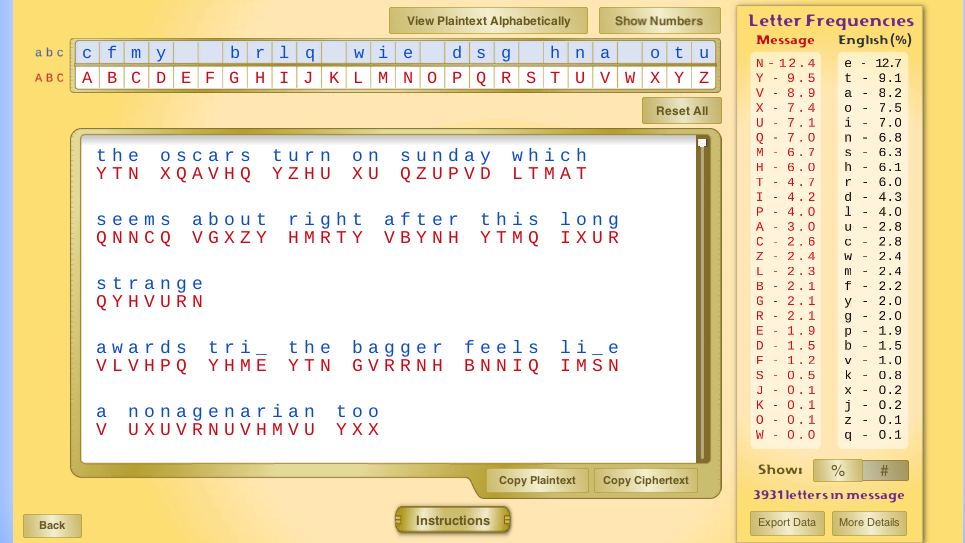
\includegraphics[scale=0.48]{c12.png}
    \end{center}{}
    \caption{Cracking the ciphertext with Crack Substitution Tool}
    \label{fig:c12}
\end{figure}

\begin{figure}[!ht]
    \begin{center}
        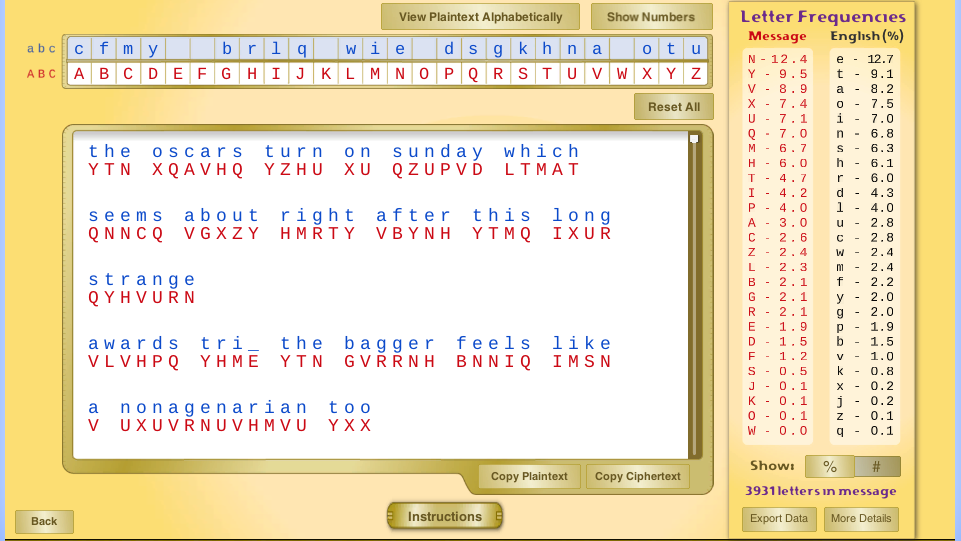
\includegraphics[scale=0.48]{c13.png}
    \end{center}{}
    \caption{Cracking the ciphertext with Crack Substitution Tool}
    \label{fig:c13}
\end{figure}

\begin{figure}[!ht]
    \begin{center}
        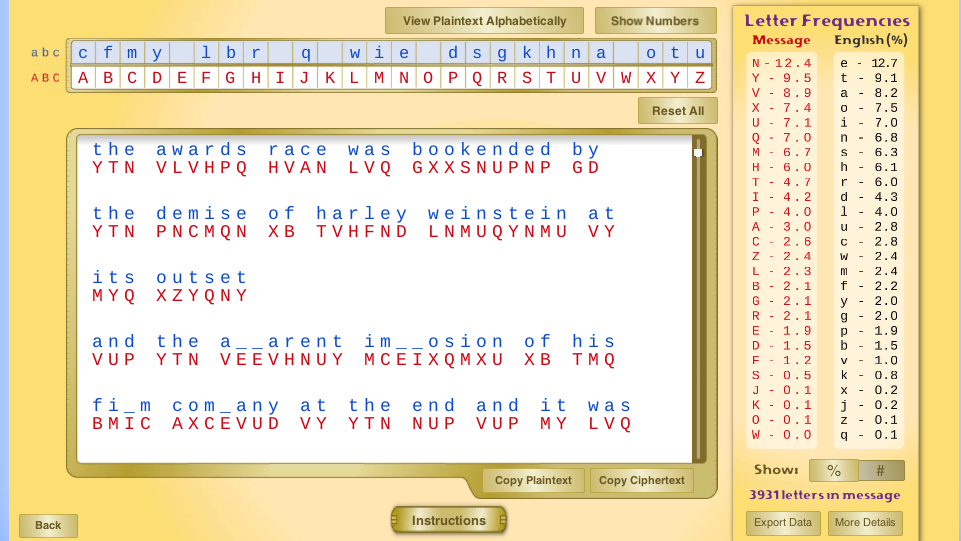
\includegraphics[scale=0.48]{c14.png}
    \end{center}{}
    \caption{Cracking the ciphertext with Crack Substitution Tool}
    \label{fig:c14}
\end{figure}

\begin{figure}[!ht]
    \begin{center}
        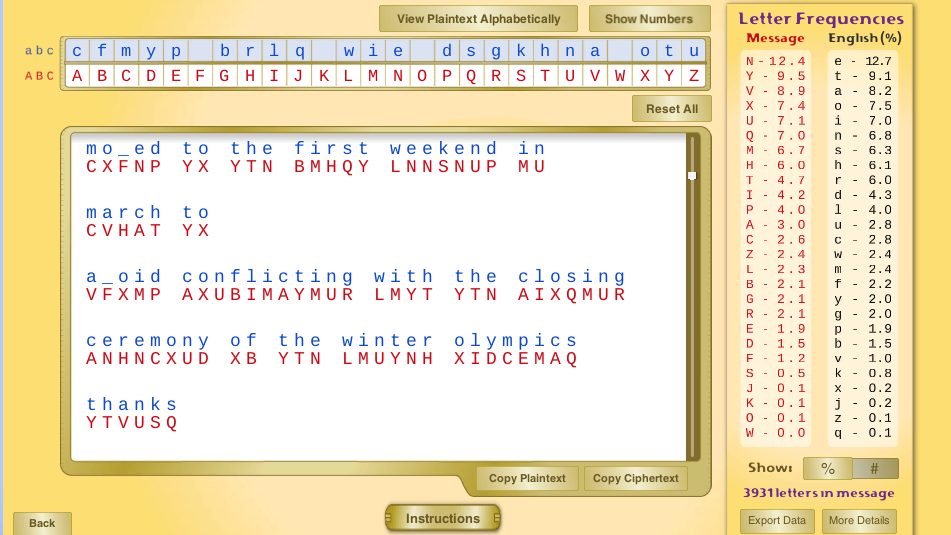
\includegraphics[scale=0.48]{c15.png}
    \end{center}{}
    \caption{Cracking the ciphertext with Crack Substitution Tool}
    \label{fig:c15}
\end{figure}

\begin{figure}[!ht]
    \begin{center}
        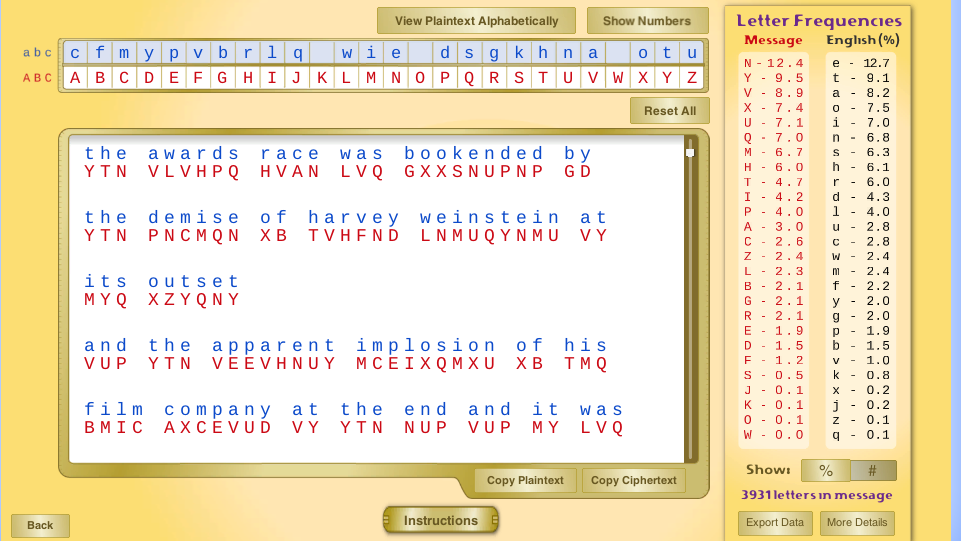
\includegraphics[scale=0.48]{c16.png}
    \end{center}{}
    \caption{Cracking the ciphertext with Crack Substitution Tool}
    \label{fig:c16}
\end{figure}

\begin{figure}[!ht]
    \begin{center}
        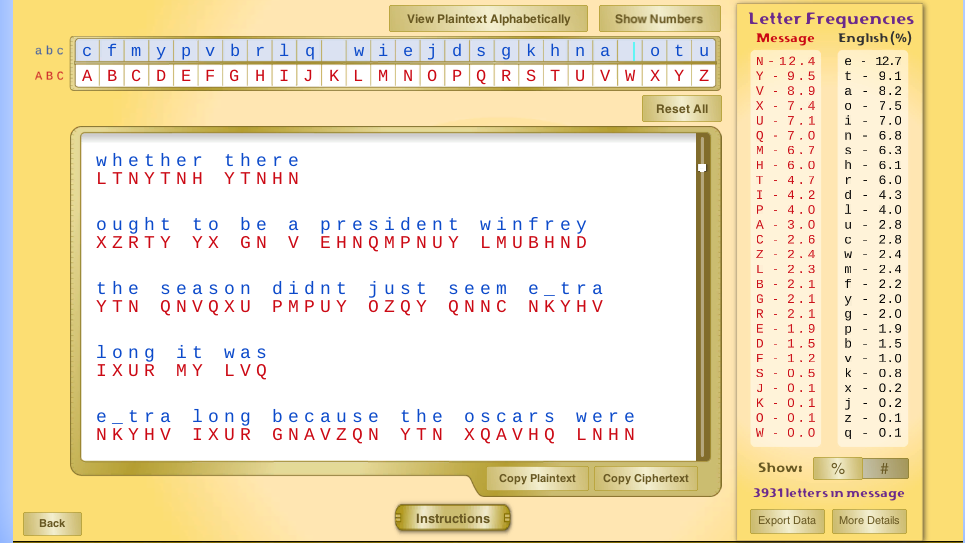
\includegraphics[scale=0.48]{c17.png}
    \end{center}{}
    \caption{Cracking the ciphertext with Crack Substitution Tool}
    \label{fig:c17}
\end{figure}

\begin{figure}[!ht]
    \begin{center}
        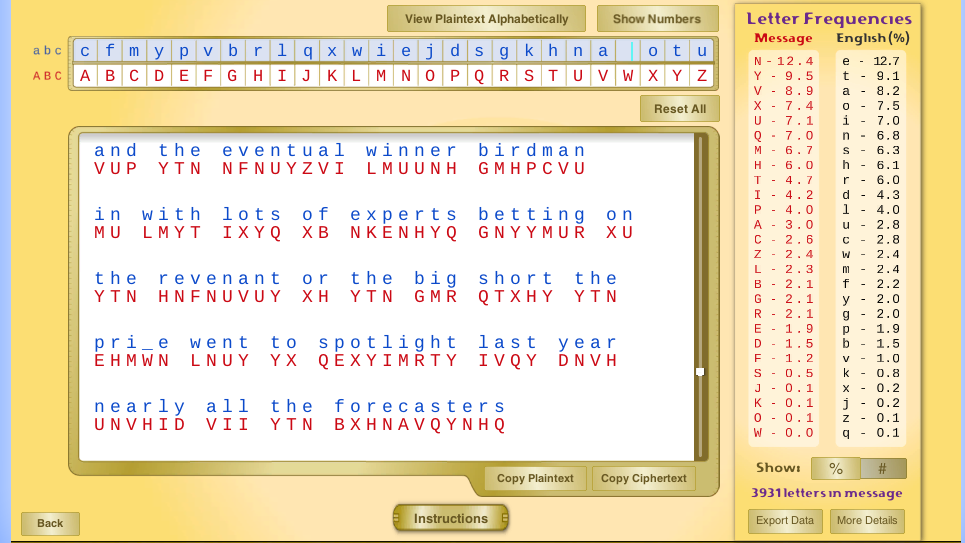
\includegraphics[scale=0.48]{c18.png}
    \end{center}{}
    \caption{Cracking the ciphertext with Crack Substitution Tool}
    \label{fig:c18}
\end{figure}

\begin{figure}[!ht]
    \begin{center}
        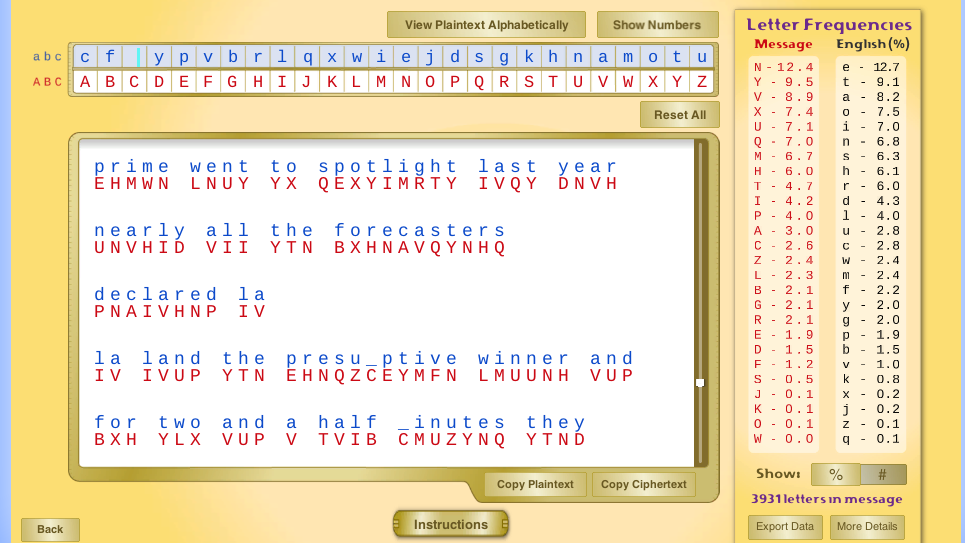
\includegraphics[scale=0.48]{c19.png}
    \end{center}{}
    \caption{Cracking the ciphertext with Crack Substitution Tool}
    \label{fig:c19}
\end{figure}

\begin{figure}[!ht]
    \begin{center}
        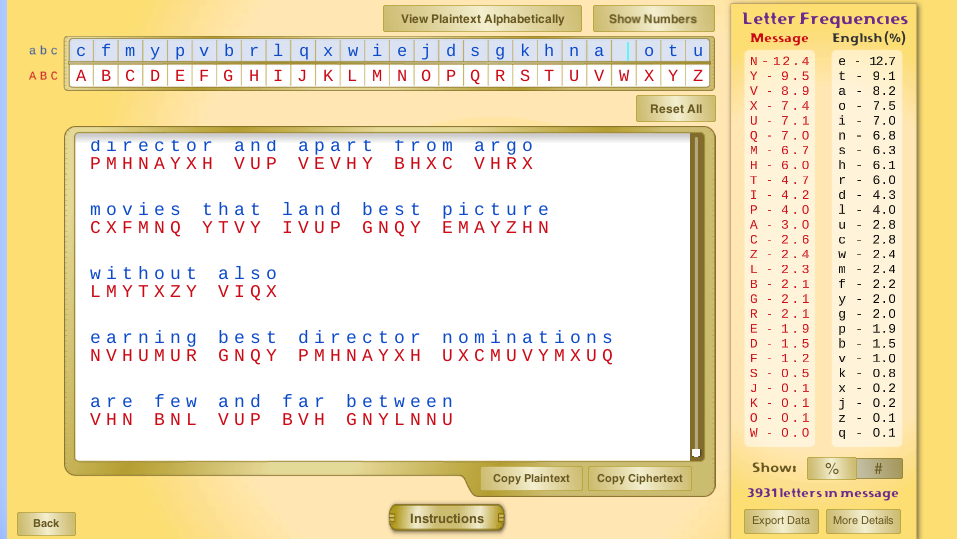
\includegraphics[scale=0.48]{c20.png}
    \end{center}{}
    \caption{Cracking the ciphertext with Crack Substitution Tool}
    \label{fig:c20}
\end{figure}

\begin{figure}[!ht]
    \begin{center}
        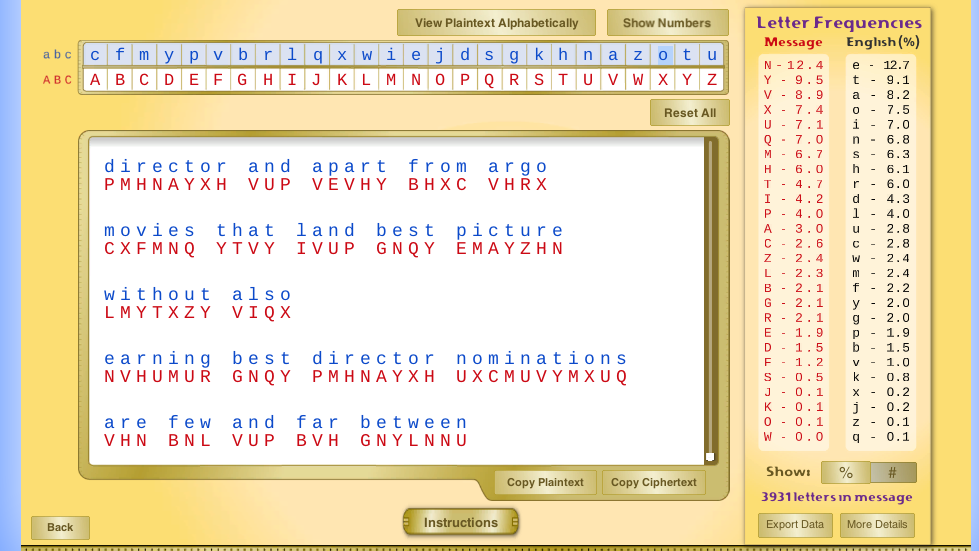
\includegraphics[scale=0.48]{c21.png}
    \end{center}{}
    \caption{Cracking the ciphertext with Crack Substitution Tool}
    \label{fig:c21}
\end{figure}











\end{document}
